\problemname{Åttaspelet}

\begin{figure}[!h]
	\centering
	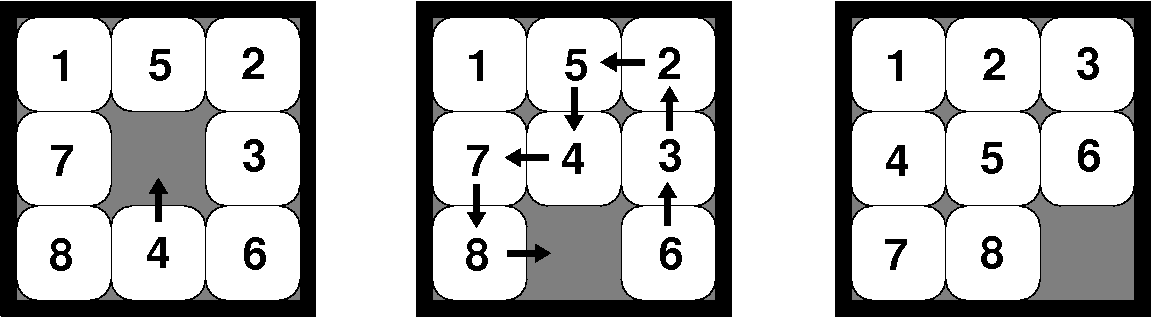
\includegraphics[width=0.55\textwidth]{figur}
	\caption{\emph{Till vänster startpositionen i det första exemplet. Pilen visar det första draget. Bilden i mitten visar ställningen efter det första draget och pilarna indikerar de återstående sju dragen som måste göras för att nå slutställningen som visas till höger.}}
\end{figure}


\emph{Åttaspelet} (ett småsyskon till det mer kända femtonspelet) är en typ av pussel som består av åtta kvadratiska brickor i en ram. Brickorna är numrerade från $1$ till $8$. Ramen rymmer $3\cdot3=9$ brickor, så det finns ett hål. Ett drag består i att man skjuter en intillliggande bricka till hålets plats. Skriv ett program som givet en startställning beräknar det minsta antalet drag som behövs för att uppnå den ordnade slutställningen som visas till höger i figuren ovan.

Tips: En godtycklig ställning är antingen olöslig (vilket inte förekommer i testfallen) eller har en lösning med högst 31 drag.

\section*{Indata}
Indatan består av en rad som innehåller bricknumret på var och en av de $9$ positionerna, eller $0$ för hålet.
Dessa beskrivs av en rad med $9$ heltal, där talen är givna i vanlig "läsordning" (översta raden först, från vänster till höger).
Varje tal mellan $0$ och $8$ kommer förekomma exakt en gång. I givna testfall kommer det alltid vara möjligt att nå slutställningen.

\section*{Utdata}
Skriv ut ett heltal: det minsta antalet drag som krävs för att uppnå slutställningen utifrån den givna positionen.

\section*{Poängsättning}
Din lösning kommer att testas på en mängd testfallsgrupper.
För att få poäng för en grupp så måste du klara alla testfall i gruppen.

\noindent
\begin{tabular}{| l | l | p{12cm} |}
  \hline
  \textbf{Grupp} & \textbf{Poäng} & \textbf{Gränser} \\ \hline
  $1$    & $40$          & Det finns en lösning som använder som mest 5 drag.  \\ \hline
  $2$    & $60$          & Inga ytterligare begränsningar.  \\ \hline
\end{tabular}
